\section{Topology optimization of a cantilever beams structure}
\label{sec:cantilever_beam}

% See the book on page 101 for results comparison

\subsection{Requests}
\label{subsec:cb_requests}

The goal of this section is to perform a topology optimization of the truss structure shown in Figure \ref{fig:truss_structure}, minimizing the compliance $C$ by acting on the cross-sectional areas of the beams.
A maximum volume constraint $V_{structure} \le V_0$ is also imposed.

\begin{figure}[H]
    \centering
    
\includegraphics[width=0.8\textwidth]{img/MATLAB/truss_cantilever/undeformed_structure.pdf}
    \caption{Unloaded truss structure to be optimized}
    \label{fig:truss_structure}
\end{figure}

As can be observed, the structure is composed of $N_{nodes} = 77$ nodes and $N_{beams} = 200$ beams.
Node indexes are indicated in the figure by the numbers reported besides each node, while the black triangles connected to some nodes represent the applied constraints.
In particular, both vertical and horizontal constrains are imposed on nodes ${47, 44, 21, 25, 57}$.

For the case at hand, we suppose to have a vertical load $F = -6000N$ applied to node $49$ (lower right corner of the structure), and the beam's Young's modulus to be $E = 210 GPa$ (steel).
Given these data, we are asked to perform the optimization for the cases reported in Table \ref{tab:cases}.

\begin{table}[H]
    \centering
    \begin{tabular}{|c|c|c|c|}
        \hline
        \textbf{Case} & \textbf{$\alpha$} & \textbf{LB $[mm^2]$} & \textbf{UB $[mm^2]$} \\
        \hline
        1             & 0.05              & 0.0001               & 800                  \\
        2             & 0.10              & 0.0001               & 800                  \\
        3             & 0.15              & 0.0001               & 800                  \\
        4             & 0.20              & 0.0001               & 800                  \\
        \hline
    \end{tabular}
    \caption{Optimization cases}
    \label{tab:cases}
\end{table}

Notice that in Table \ref{tab:cases}, the abbreviations LB and UB stand for Lower Bound and Upper Bound, respectively.

The parameter $\alpha$ is the volume fraction of the structure, defined as $\alpha = \frac{V_0}{V_{max}}$, where $V_{max} = \text{UB} \sum_{j=1}^{N_{beams}} l_j$ is the maximum volume of the structure.



\subsection{Solution procedure}
\label{subsec:cb_solution_procedure}

At first, we recognize that the given optimization problem is a compliance minimization problem, and so we can use the theoretical background presented in Section \ref{subsubsec:compliance_minimization_problem}.

In addition to what has already been discussed in Section \ref{subsubsec:compliance_minimization_problem}, we adopt some additional naming conventions that will also be used in the code implementation.
In particular, in Equation \ref{eq:conlin_compliance_minimization_problem}, we define the following quantities:

\begin{equation}
    \begin{aligned}
        f^{(C, k)} & = f(\bm{x}^{(k)}) + \sum_{j \in \Omega_-} \frac{\partial f(\bm{x}^{(k)})}{\partial x_j} \frac{x_j^{(k)}(x_j - x_j^{(k)})}{x_j} \\
                   & = r_0^k + \sum_{j \in \Omega_-} \frac{q_{0j}^k}{x_j}
    \end{aligned}
\end{equation}

Where:

\begin{equation}
    \begin{aligned}
        r_0^k    & = f(\bm{x}^{(k)}) - \sum_{j \in \Omega_-}  x_j^k u_j^T(\bm{x}^k) \bm{K}_j^0 u_j^T(\bm{x}^k) \\
        q_{0j}^k & = u_j^T(\bm{x}^k) \bm{K}_j^0 u_j^T(\bm{x}^k) (x_j^k)^2
    \end{aligned}
\end{equation}

Based on these definitions, we can redefine both the optimization problem $(P)_{nf}$ and the Lagrangian function $\mathcal{L}^{k}(\bm{x}, \bm{\lambda})$ as follows:

\begin{equation}
    \begin{aligned}
        (P)_{nf}^C \quad & \begin{cases}
                               \min_{\bm{x}} & f^{(C, k)} = r_0^k + \sum_{j \in \Omega_-} \frac{q_{0j}^k}{x_j} \\
                               \text{s. t.}  & \sum_{j=1}^{n} l_j x_j - V_{max} \leq 0                         \\
                                             & \bm{x} \in \Omega
                           \end{cases} \\
                         & \Omega := \{ \bm{x} \in \mathbb{R}^n \mid x_j^{min} < x_j \le x_j^{max}, \quad j = 1, \dots, n \}
    \end{aligned}
\end{equation}

\begin{equation}
    \mathcal{L}^{k}(\bm{x}, \bm{\lambda}) = r_0^k + \sum_{j \in \Omega_-} (\frac{q_{0j}^k}{x_j} + \lambda_j l_j x_j) - \lambda V_{max}
\end{equation}

Also, the solution of the dual optimization problem $(D)_{nf}$ can be found by solving the following equation:

\begin{equation}
    \frac{\partial \mathcal{L}^k}{\partial x_j} = - \frac{q_{0j}^k}{x_j} + \lambda_j l_j = 0 \rightarrow x_j^* = \sqrt{\frac{q_{0j}^k}{\lambda_j l_j}}
\end{equation}

Notice however that the solution given by the equation above may not respect the constraints $x_j^{min} < x_j < x_j^{max}$.
In this case, we can use the following projection operator to find the optimal solution:

\begin{equation}
    x_j^{(k+1)}(\lambda) = \begin{cases}
        x_j^*     & \text{if } x_j^* \in [x_j^{min}, x_j^{max}] \\
        x_j^{min} & \text{if } x_j^* < x_j^{min}                \\
        x_j^{max} & \text{if } x_j^* > x_j^{max}
    \end{cases}
\end{equation}

Finally, we can use the following update rule to find the optimal value of the Lagrangian multiplier $\lambda$:

\begin{equation}
    \frac{\partial \psi^k(\lambda)}{\partial \lambda} = \sum_{j \in \Omega_-} l_j x_j^{(k+1)} - V_{max} = 0
\end{equation}

So basically, one can solve for the Lagrangian multiplier $\lambda$ by finding numerically the root of the equation above.
Once the optimal value of $\lambda$ is found, we can update the design variables $\bm{x}$ using the projection operator defined above, and then update the Lagrangian function $\mathcal{L}^{k}(\bm{x}, \bm{\lambda})$.
This iterative procedure can be repeated until convergence is reached.

One can refer to the MATLAB code provided in the Appendix \ref{lst:core} for the implementation of the solution procedure described above.



\subsection{Results}
\label{subsec:cb_results}

Based on the solution procedure described in Section \ref{subsec:cb_solution_procedure}, the results of the topology optimization of the truss structure for the cases reported in Table \ref{tab:cases} are shown in Figures \ref{fig:cb_case1}, \ref{fig:cb_case2}, \ref{fig:cb_case3}, and \ref{fig:cb_case4}.

\begin{figure}[H]
    \centering
    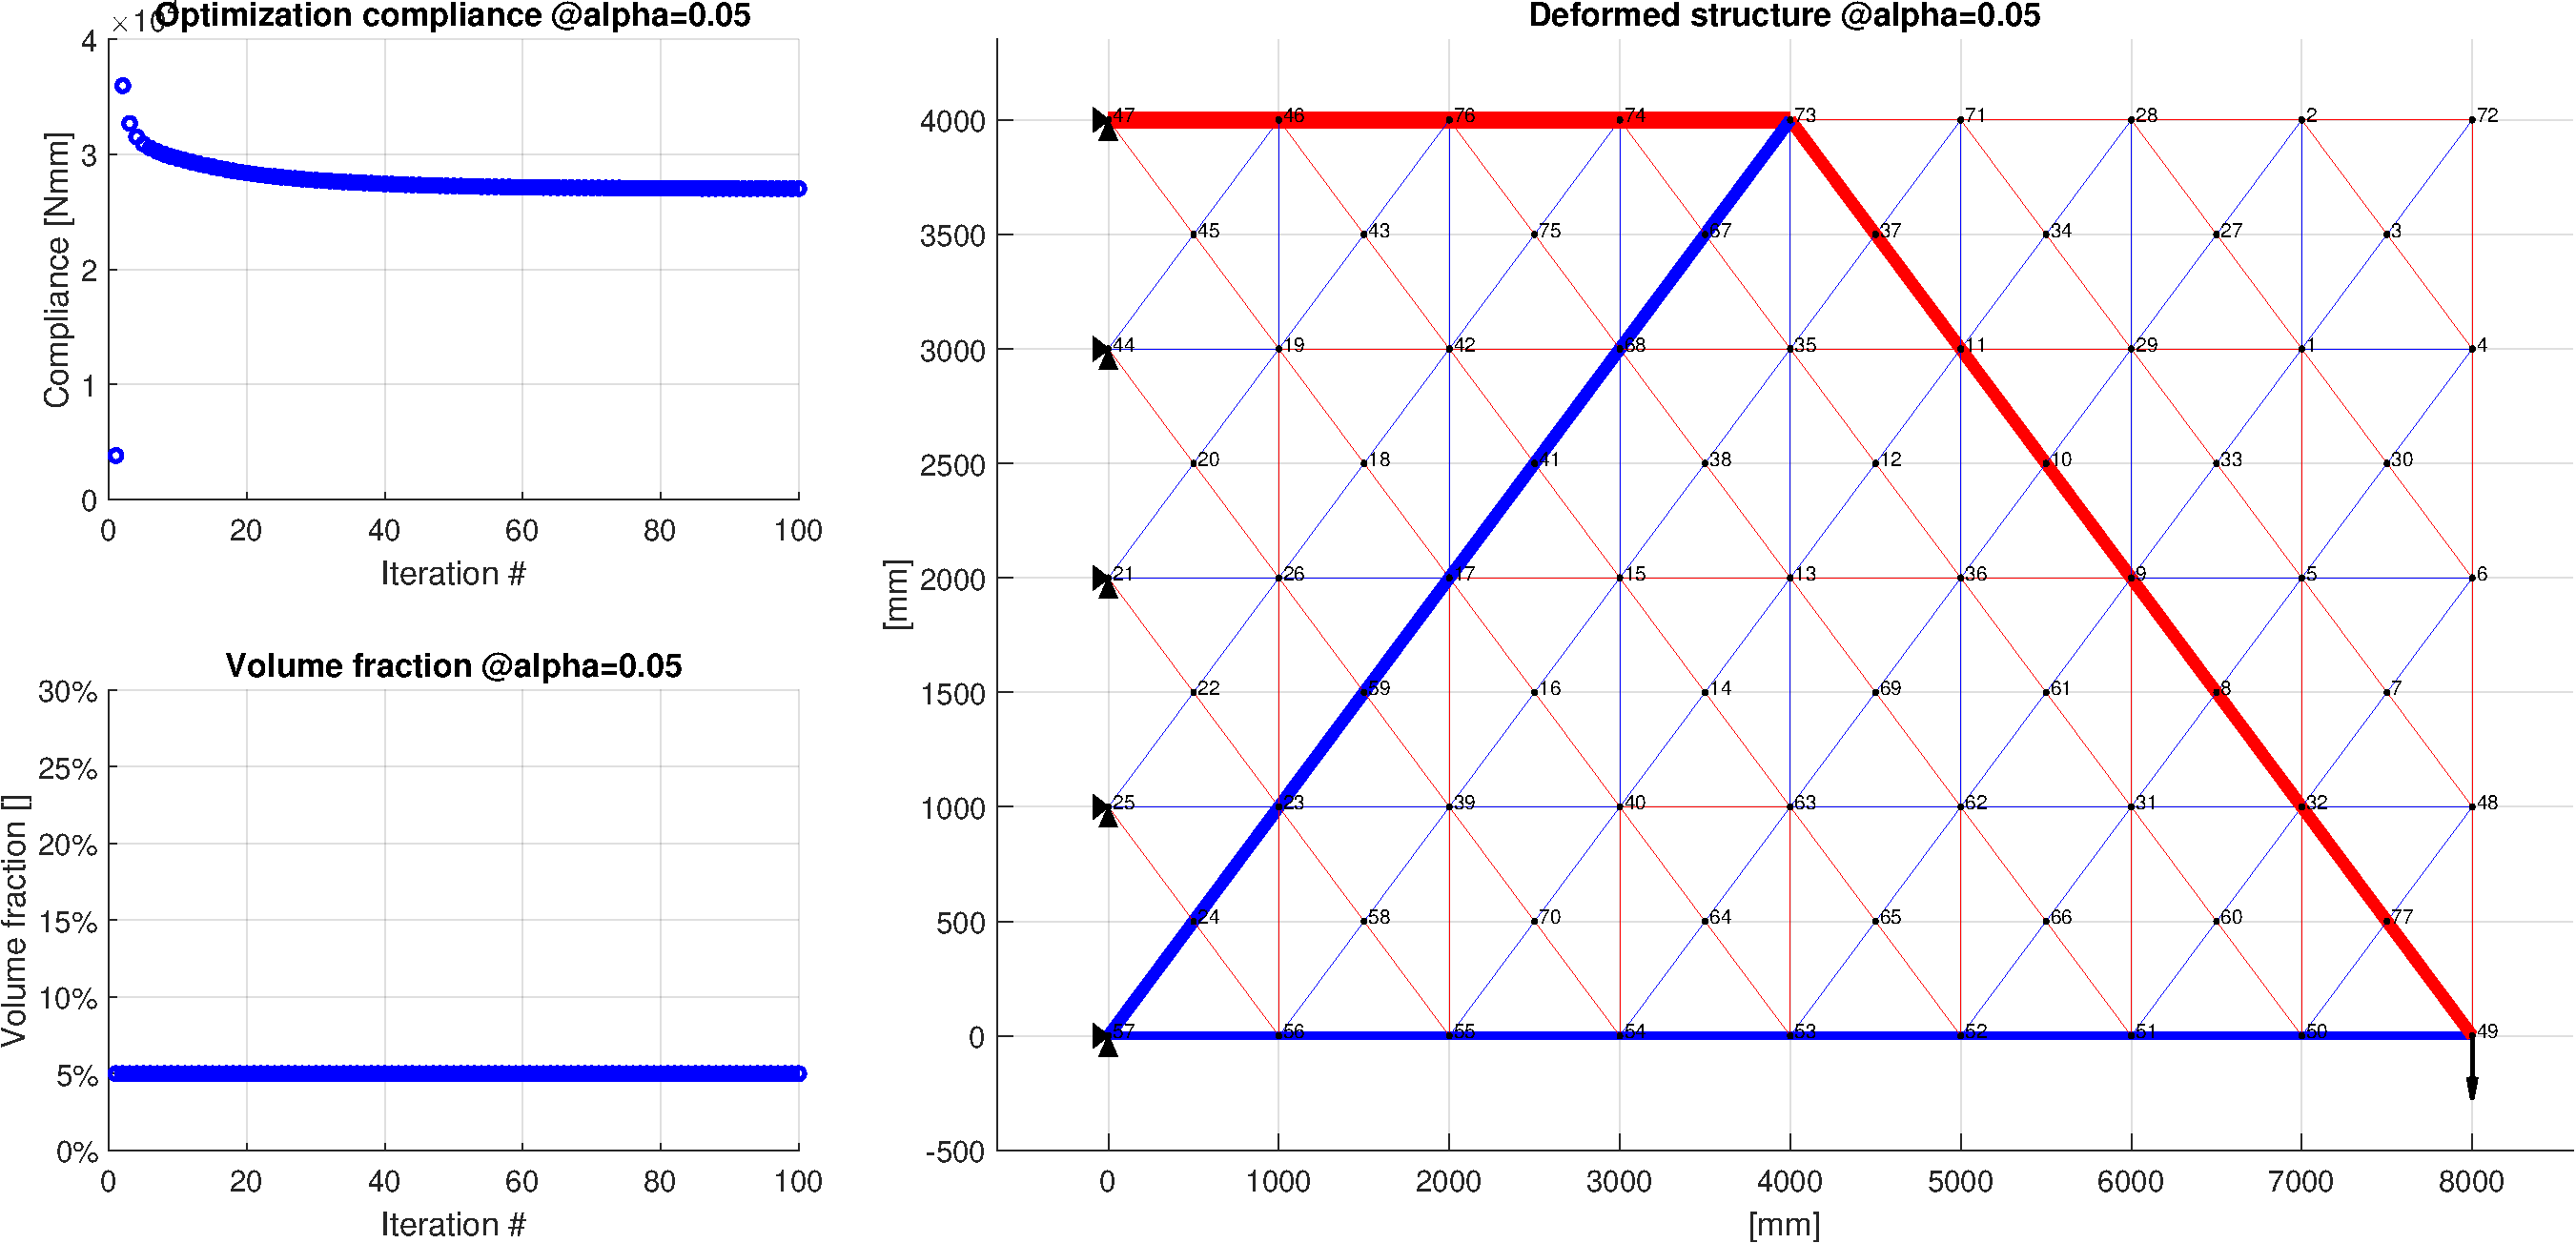
\includegraphics[width=1\textwidth]{img/MATLAB/truss_cantilever/results_alpha5.pdf}
    \caption{Optimized truss structure for Case 1 ($\alpha = 0.05$)}
    \label{fig:cb_case1}
\end{figure}

\begin{figure}[H]
    \centering
    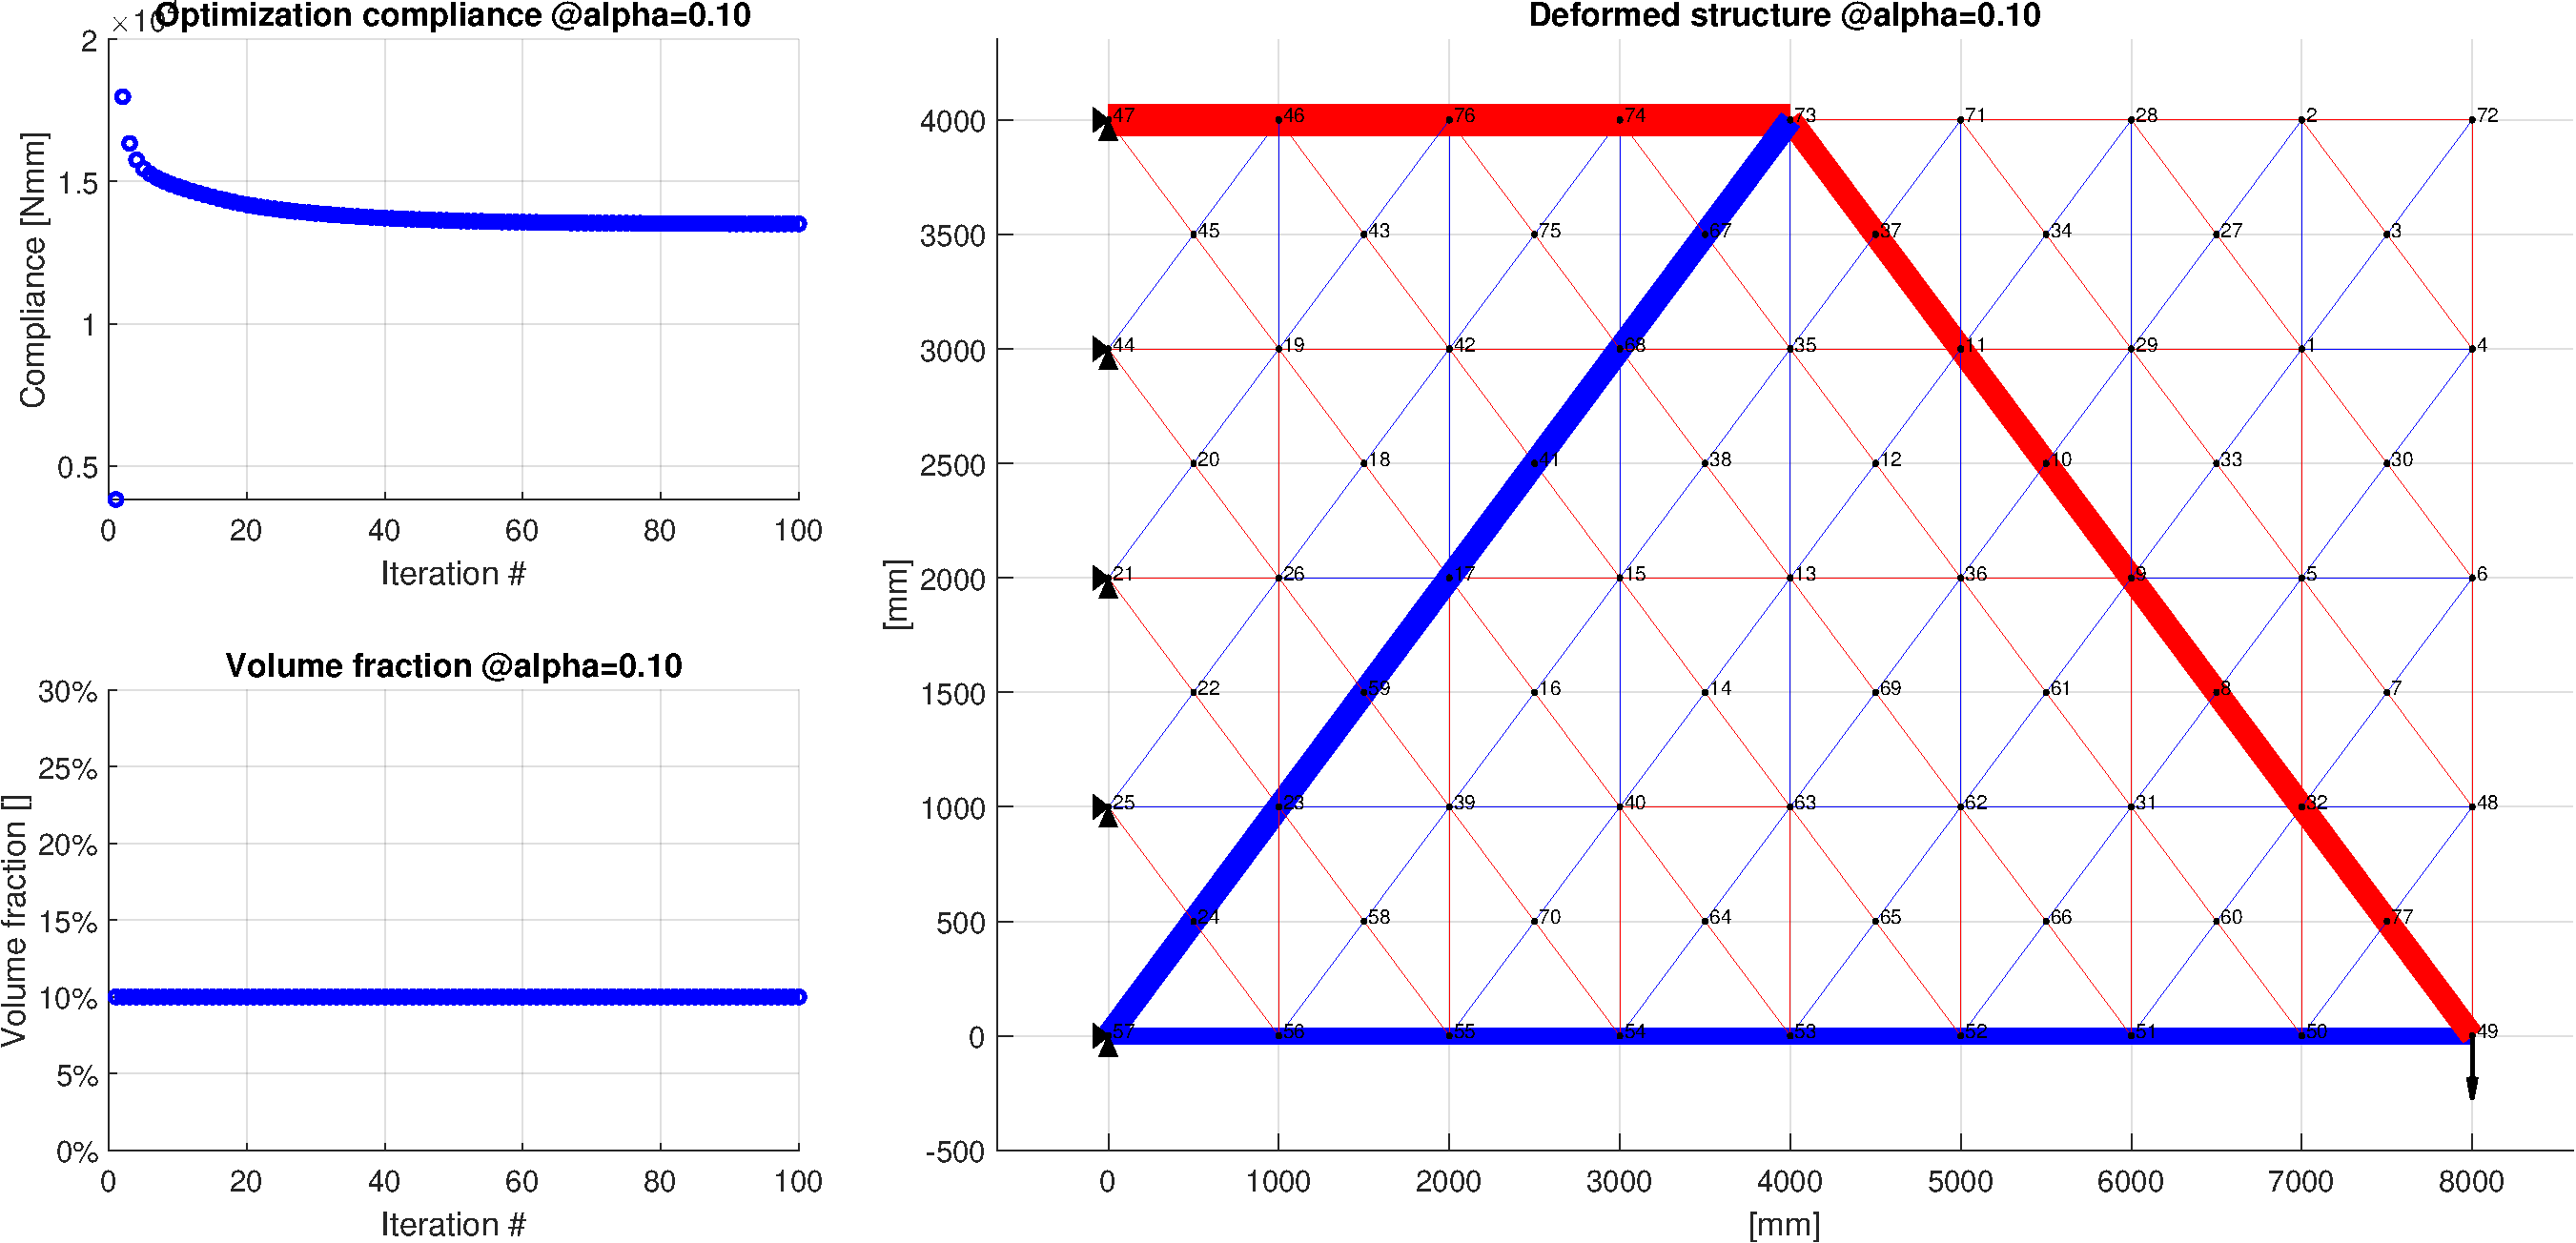
\includegraphics[width=1\textwidth]{img/MATLAB/truss_cantilever/results_alpha10.pdf}
    \caption{Optimized truss structure for Case 2 ($\alpha = 0.10$)}
    \label{fig:cb_case2}
\end{figure}

\begin{figure}[H]
    \centering
    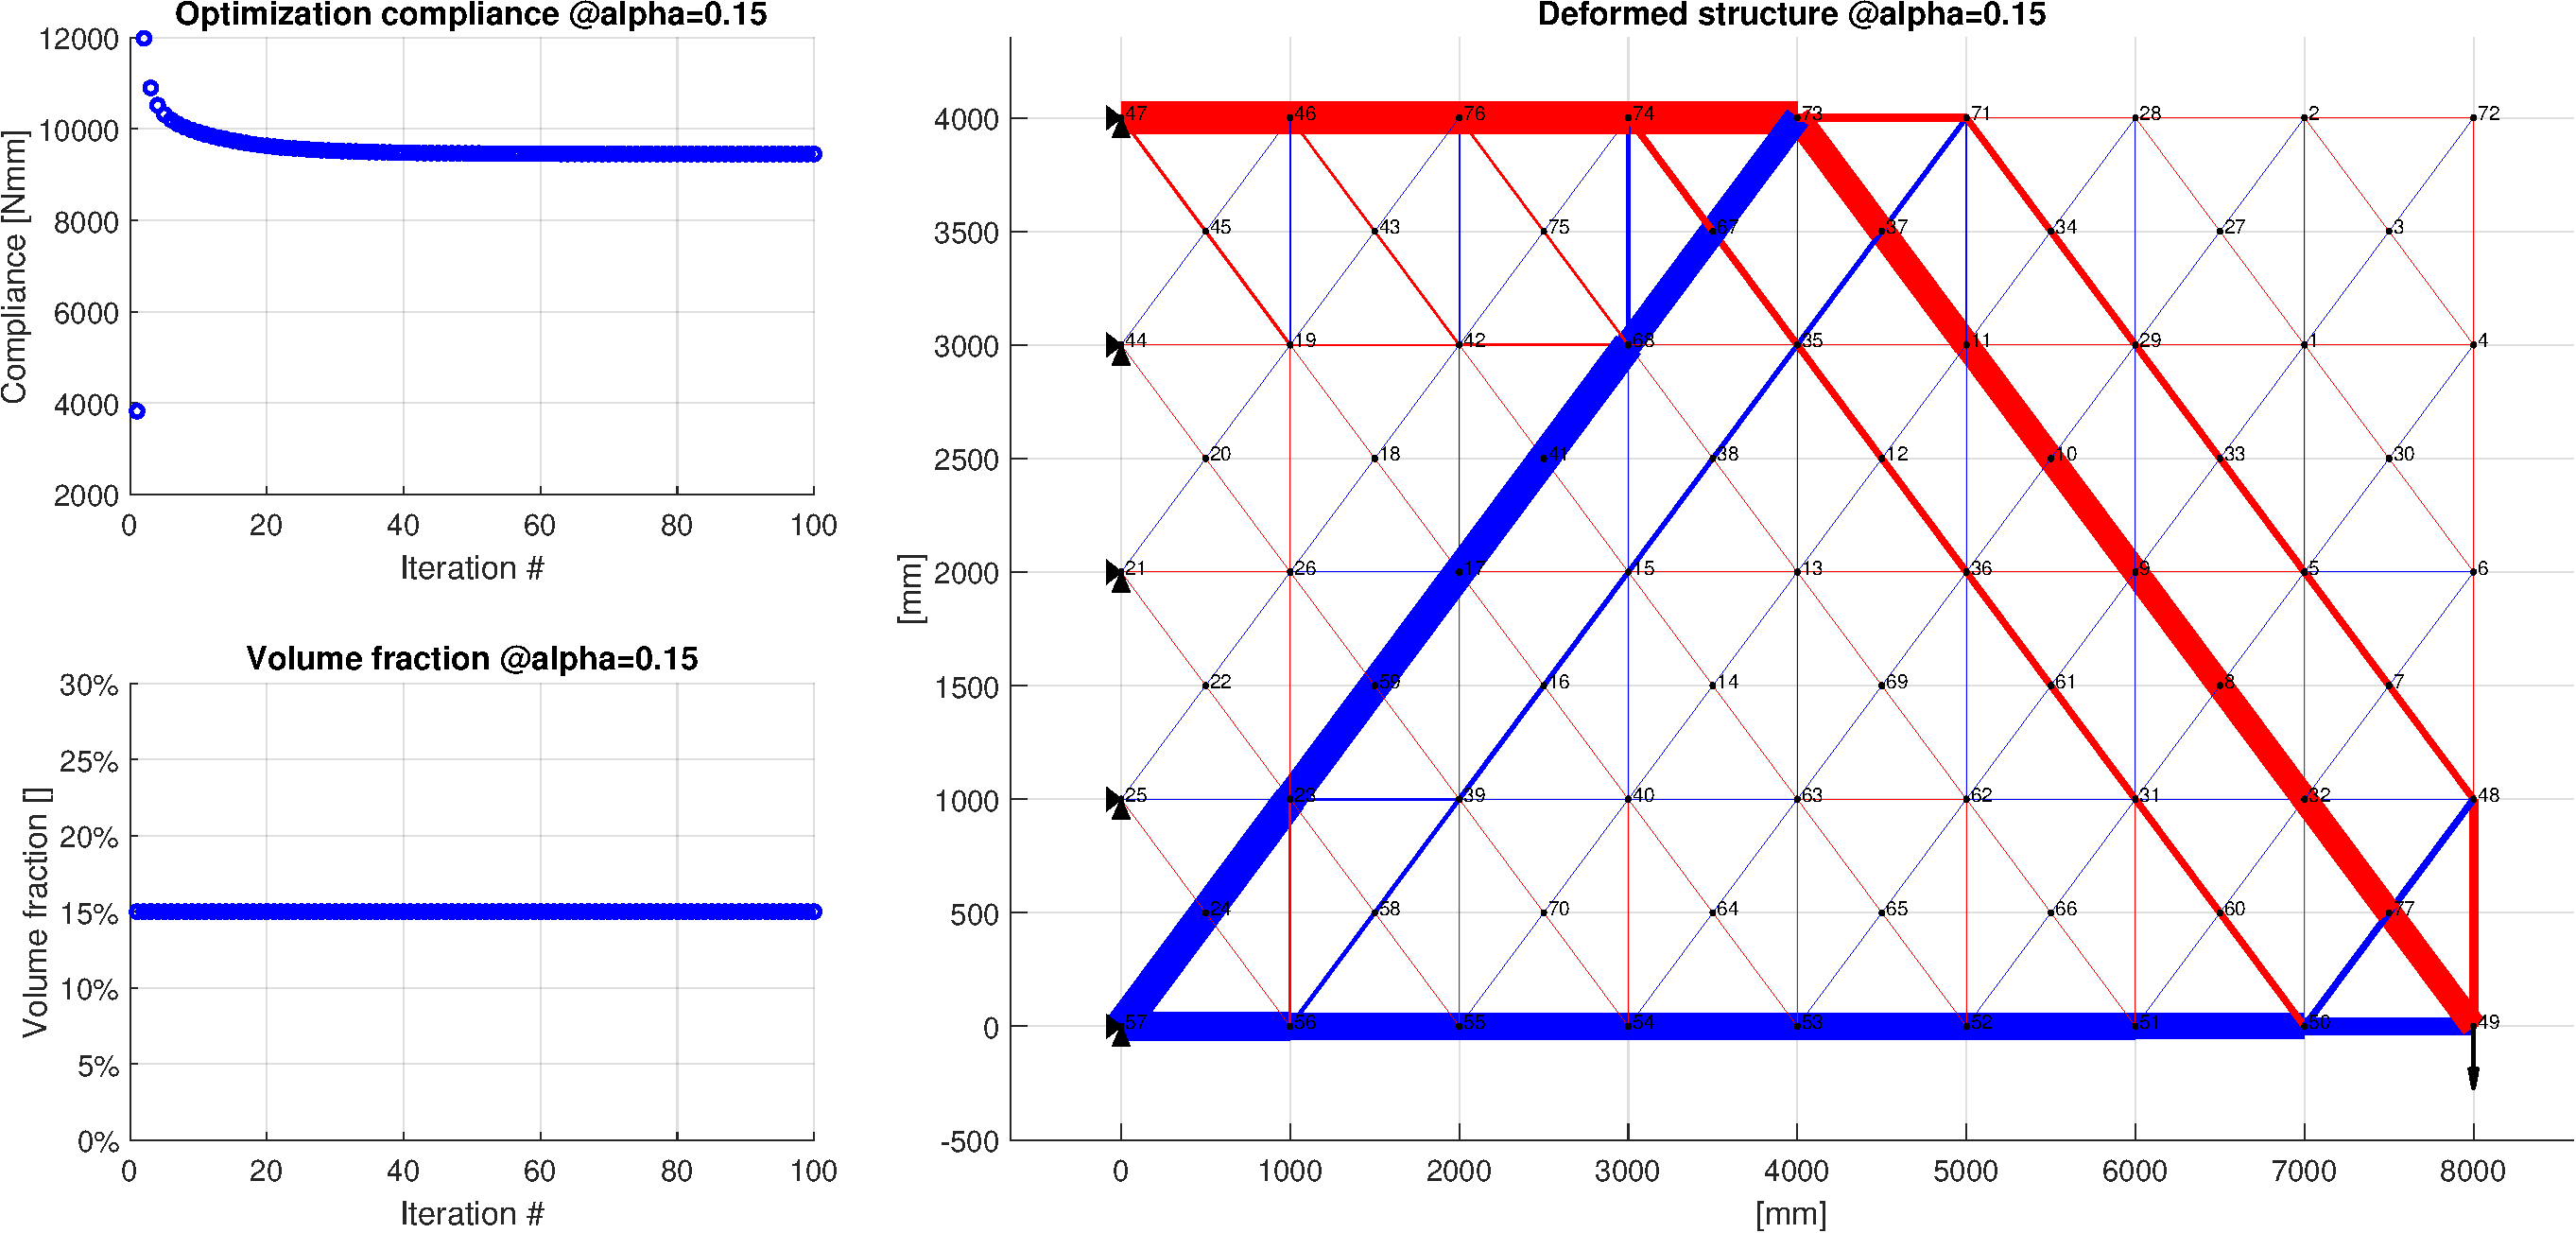
\includegraphics[width=1\textwidth]{img/MATLAB/truss_cantilever/results_alpha15.pdf}
    \caption{Optimized truss structure for Case 3 ($\alpha = 0.15$)}
    \label{fig:cb_case3}
\end{figure}

\begin{figure}[H]
    \centering
    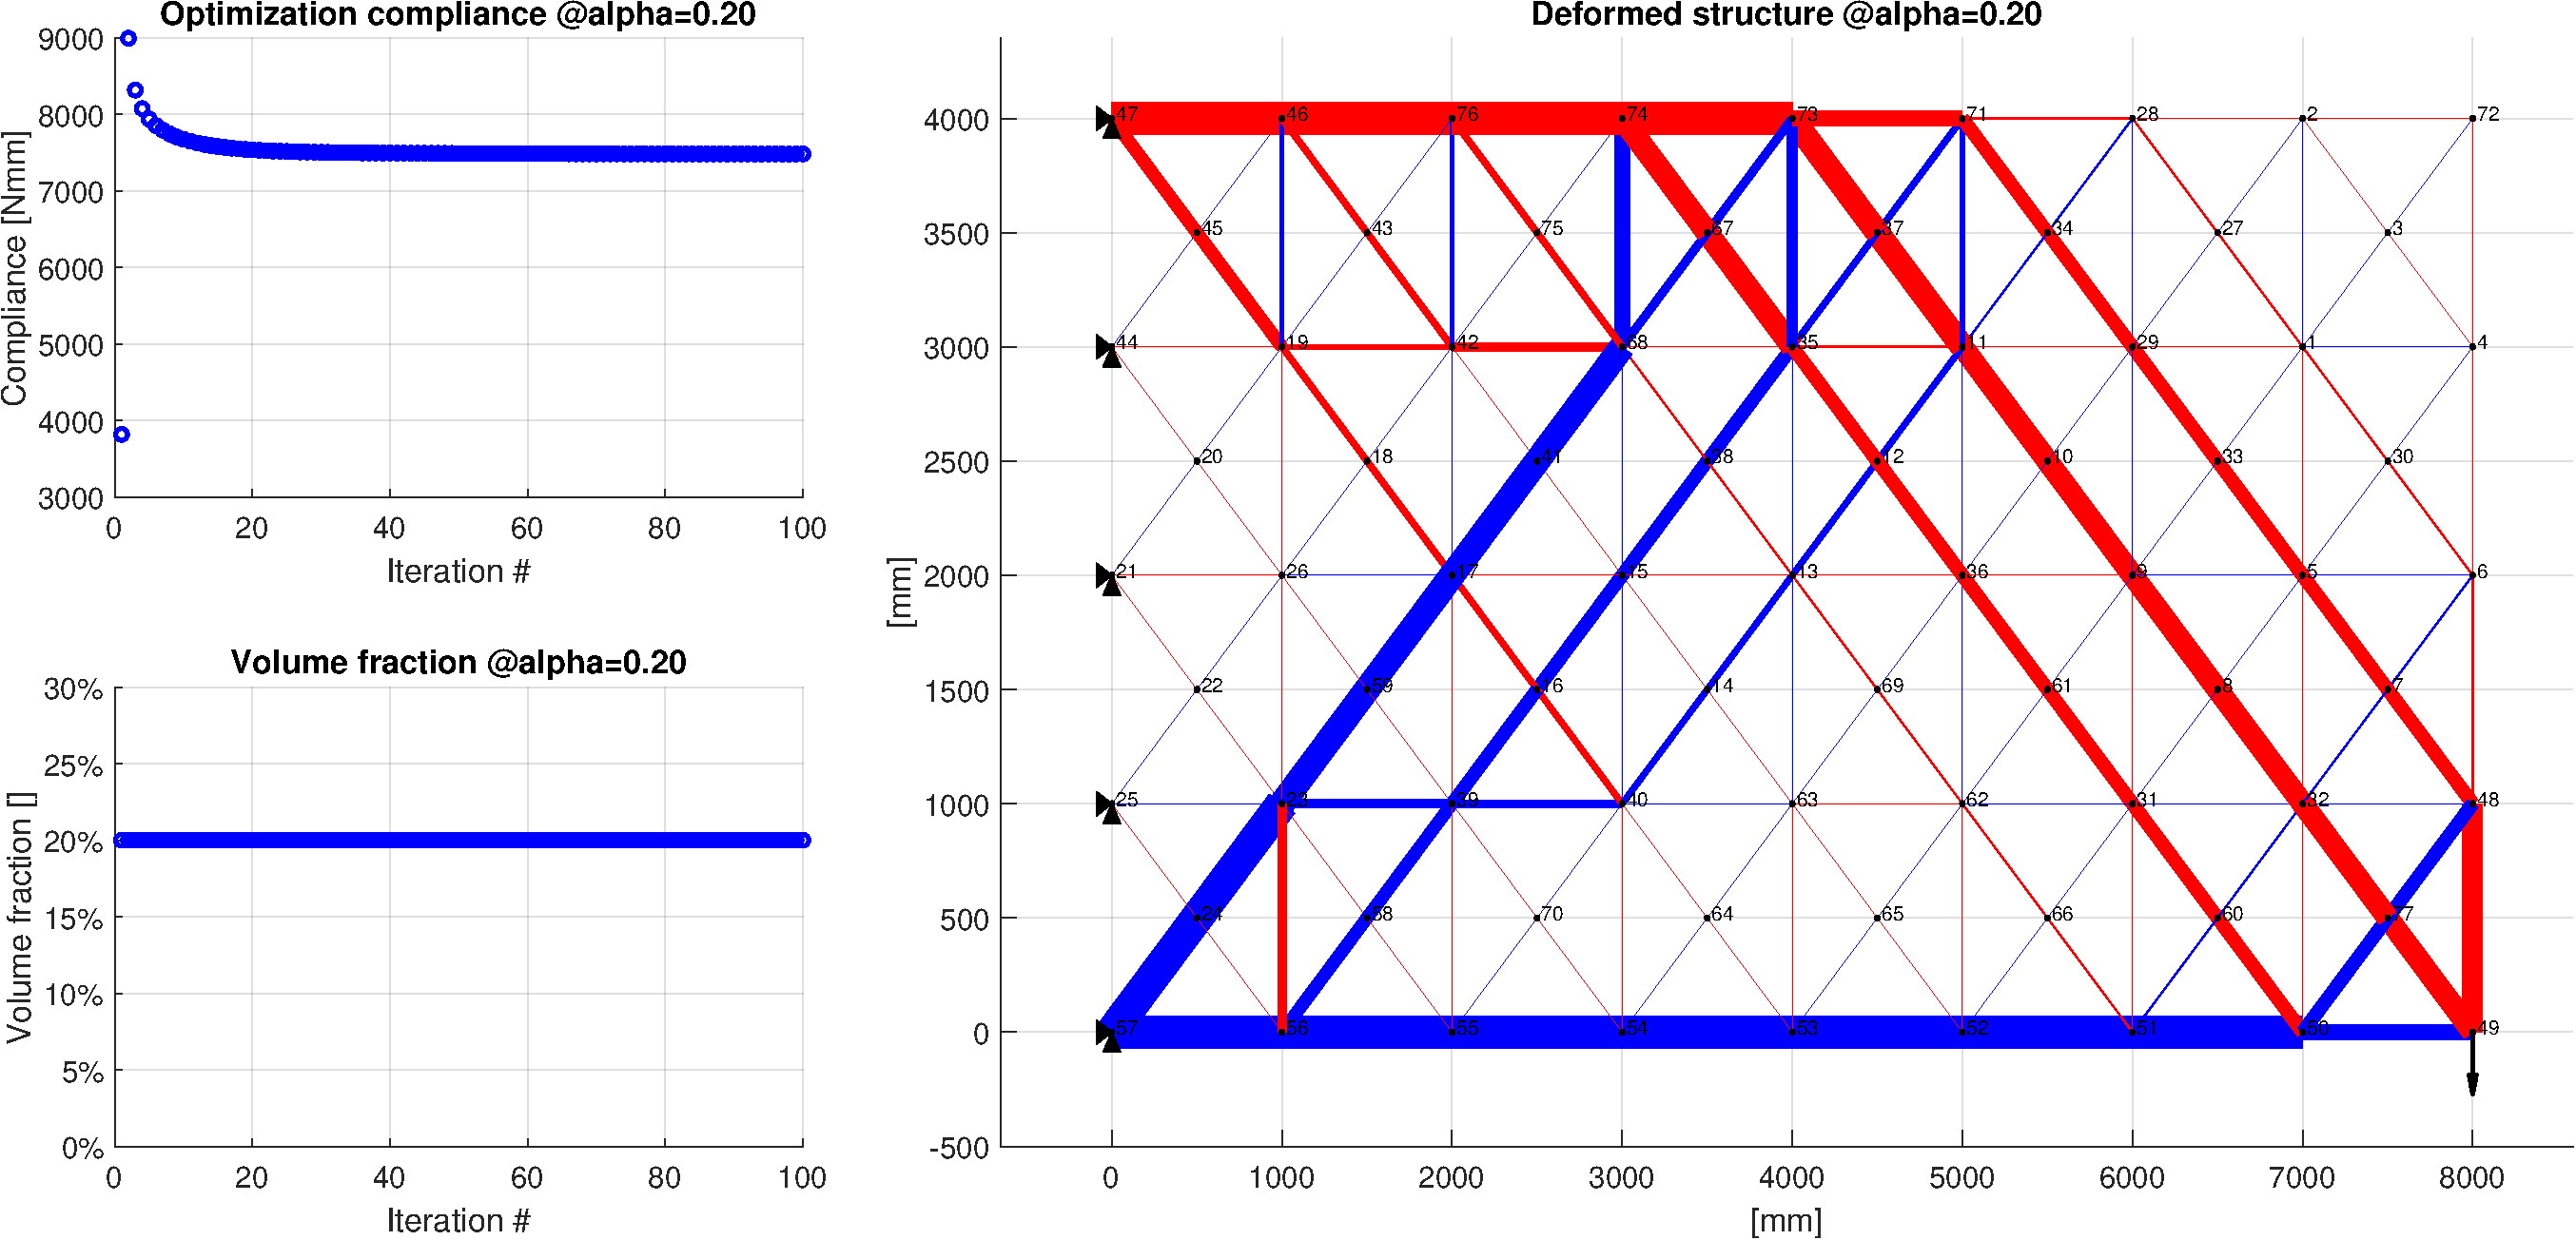
\includegraphics[width=1\textwidth]{img/MATLAB/truss_cantilever/results_alpha20.pdf}
    \caption{Optimized truss structure for Case 4 ($\alpha = 0.20$)}
    \label{fig:cb_case4}
\end{figure}

One can clearly notice how the volume fraction $\alpha$ affects the topology of the optimized structure.
In particular, larger values of $\alpha$ lead to a denser structure, with more beams contributing to the load-bearing capacity of the structure.
On the other hand, smaller values of $\alpha$ lead to a stiffer structure, with increased compliance values.

Finally, as requested by the project, we report in the following table the cross-sectional areas and the stresses acting in elements $[64, 77, 82]$ for the cases reported in Table \ref{tab:cases}.

\begin{table}[H]
    \centering

    \begin{tabular}{|c|c|c|c|}
        \hline

        \textbf{Case}      & \textbf{Element} & \textbf{Area $[mm^2]$} & \textbf{Stress $[MPa]$} \\
        \hline
        \multirow{3}{*}{1} & 64               & 406.27                 & +29.54                  \\
                           & 77               & 203.14                 & -29.54                  \\
                           & 82               & 287.27                 & -29.54                  \\
        \hline
        \multirow{3}{*}{2} & 64               & 800.00                 & +15.00                  \\
                           & 77               & 408.36                 & -14.69                  \\
                           & 82               & 577.50                 & -14.69                  \\
        \hline
        \multirow{3}{*}{3} & 64               & 800.00                 & +14.42                  \\
                           & 77               & 653.68                 & -9.18                   \\
                           & 82               & 800.00                 & -9.31                   \\
        \hline
        \multirow{3}{*}{4} & 64               & 800.00                 & +13.17                  \\
                           & 77               & 800.00                 & -7.50                   \\
                           & 82               & 800.00                 & -8.02                   \\
        \hline
    \end{tabular}

    \caption{Cross-sectional areas and stresses for elements $[64, 77, 82]$}
    \label{tab:cb_results}

\end{table}

From Table \ref{tab:cb_results}, it can be observed that when the cross-sectional areas of a given element remain within the optimization constraint bounds (i.e., lower bound (LB) and upper bound (UB)), the stresses acting in those elements become equal.
This phenomenon occurs because the Lagrangian multiplier is directly proportional to the square stress in cases where the element area stays within these specified bounds.
That is:

\begin{equation}
    \lambda_j = \frac{\sigma_j^2}{E} \rightarrow \sigma_j = \sqrt{E \lambda_j}
\end{equation}